\documentclass[10pt]{beamer}

\mode<presentation>
{
  \usetheme[height=1.25cm]{Madrid}
  \setbeamertemplate{navigation symbols}{}
  \setbeamercolor{alerted text}{fg=illini}
}
\usebackgroundtemplate{
\includegraphics[width=\paperwidth,height=\paperheight]{uc-background}}

\usepackage[english]{babel}
\usepackage{epsfig,subfigure,bm}
\usepackage{multimedia}
\usepackage{psfrag}
\usepackage{animate}

%%%%%% Begin of my macros and options

\setbeamertemplate{section in toc shaded}[default][55]
\setbeamertemplate{subsection in toc shaded}[default][55]
\setbeamercolor{block title}{fg=white,bg=illini}
\setbeamercolor{block body}{fg=black,bg=mygrey}

\setbeamercolor{emphprimary}{fg=CBlue}
\setbeamercolor{emphsecondary}{fg=illini}
\setbeamercolor{emphtertiary}{fg=mygreen}
\definecolor{darkForestGreen}{rgb}{.1,1,.1}
\definecolor{veryLightGray}{rgb}{.9,.9,.9}
\definecolor{greenApple}{rgb}{.3,.9,.3}

\setbeamercolor{frametitle}{bg=CBlue}   
\setbeamercolor{title}{bg=CBlue}

\usepackage{amsmath,amssymb,amsxtra,amsthm}
\usepackage{algorithm,algorithmic}
\usepackage{natbib}
\usepackage{bibentry}
\usepackage{xspace}
\usepackage{changepage}

\pdfmapfile{+sansmathaccent.map}

\definecolor{myblue}{rgb}{.2,.2,.7}
\definecolor{myred}{rgb}{.7,.2,.2}
\definecolor{mygreen}{rgb}{.2,.7,.2}
\definecolor{mygrey}{rgb}{0.9,0.9,0.9}
\definecolor{CBlue}{cmyk}{1,0.25,0,0}
\definecolor{illini}{rgb}{0.98,0.4,0.05}
\definecolor{black}{cmyk}{0,0,0,1}

\newcommand{\myemph}[1]{{\usebeamercolor[fg]{emphprimary}
    \textbf{#1}}}
\newcommand{\myemphalt}[1]{{\usebeamercolor[fg]{emphsecondary}
    \textbf{#1}}}

\graphicspath{{figs/}}

\title[Math for Robotics] % (optional, use only with long paper titles)
{CSE276C - Linear Systems of Equations}

\author[H.~I. Christensen] % (optional, use only with lots of authors)
{Henrik I.~Christensen}
% - Give the names in the same order as the appear in the paper.  -
% Use the \inst{?} command only if the authors have different
% affiliation.

\institute[UCSD] % (optional, but mostly needed)
{
  \begin{minipage}[c]{.2\textwidth}
    
\includegraphics[width=.65\linewidth]{ucsealnew}%
  \end{minipage}%
  \begin{minipage}[c]{.6\textwidth}
    \small
%%    \begin{center}
      Computer Science and Engineering\\
      University of California, San Diego\\
      \myemph{\url{http://cri.ucsd.edu}}\\          
%%    \end{center}

  \end{minipage}
%%  \vspace*{1ex}
}
%% - Use the \inst command only if there are several affiliations.
%% - Keep it simple, no one is interested in your street address.

\bigskip

\date[Sep 2021]% (optional, should be abbreviation of conference name)
{\small%
  September 2021}

\begin{document}
  
\nobibliography{/Users/hic/Dropbox/bibliography/bib-file}
\bibliographystyle{plain}

\begin{frame}[plain]
  \titlepage
\end{frame}


\begin{frame}
  \frametitle{Outline}
  \begin{itemize}
  \item Linear Systems of Equations
  \item Solution Techniques - Gauss Jordan
  \item Matrix Decomposition
  \item Matrix Factorization
  \item Singular Value Decomposition
  \item Rank and sensitivity
  \end{itemize}
\end{frame}

\begin{frame}
  \frametitle{Material}
  \begin{itemize}
  \item Numerical Recipes: Chapter  2
  \item Math for ML: Chapter 2.1-2.3
  \end{itemize}
\end{frame}

\begin{frame}
  \frametitle{Example: Camera calibration}
  \centerline{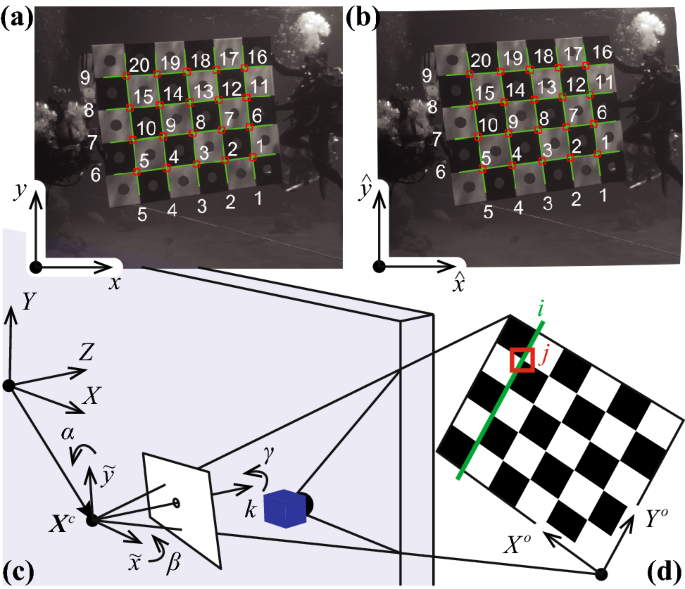
\includegraphics[height=6.5cm]{calibration}}
\end{frame}

\begin{frame}
  \frametitle{Example: Plane Estimation}
  \centerline{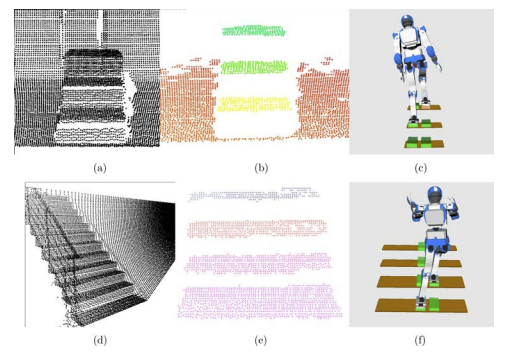
\includegraphics[height=6.5cm]{plane-estimation}}
\end{frame}

\begin{frame}
  \frametitle{Linear Systems of Equations}
  \begin{itemize}
  \item One of the most basic tasks is solve for a set of unknowns
    \[
      \begin{array}{ccc}
        a_{00} x_0 + a_{01} x_1 + a_{02} x_2 + \ldots + a_{0n-1} x_{n-1} & = & b_0\\
        a_{10} x_0 + a_{11} x_1 + a_{12} x_2 + \ldots + a_{1n-1} x_{n-1} & = & b_1\\
        \vdots && \\
        a_{m-10} x_0 + a_{m-11} x_1 + a_{m-12} x_2 + \ldots + a_{m-1n-1} x_{n-1} & = & b_{m-1}\\
      \end{array}
    \]
    \pause
  \item which we can rewrite
    \[
      \mathbf{A} \vec{x} = \vec{b}
    \]
    where
    \[
      \mathbf{A} = \left(
        \begin{array}{ccccc}
          a_{00} & a_{01} & a_{01} & \cdots & a_{0n-1} \\
          a_{10} & a_{11} & a_{11} & \cdots & a_{1n-1} \\
          & &  \vdots & & \\
          a_{m-10} & a_{m-11} & a_{m-11} & \cdots & a_{m-1n-1} \\
        \end{array}\right), 
      \vspace{1cm} 
      \vec{b} = \left(
        \begin{array}{c}
          b_0 \\ b_1 \\ b_2 \\ \vdots \\ b_{m-1} \\
        \end{array}\right)
    \]
  \end{itemize}
\end{frame}

\begin{frame}
  \frametitle{Matrix Properties}
  \begin{itemize}
  \item Given an $m \times n$ matrix A we define
    \begin{itemize}
    \item Column space - Linear combination of columns
    \item Row space - Linear combination of row
    \end{itemize}
  \item We can consider A a mapping:
    \[
      A: R^n \rightarrow R^m
    \]
    \[
      \left(
        \begin{array}{c}
          x_0 \\ x_1 \\ \vdots \\ x_{n-1} \\
        \end{array}
      \right) \rightarrow
      \left(
        \begin{array}{c}
          b_0 \\ b_1 \\ \vdots \\ b_{m-1} \\
        \end{array}
      \right) =
      \mathbf{A}
      \left(
        \begin{array}{c}
          x_0 \\ x_1 \\ \vdots \\ x_{n-1} \\
        \end{array}
      \right)
    \]
  \item Column space of A is vector subspace of $R^m$ that image
    vectors under A
  \end{itemize}
\end{frame}

\begin{frame}
  \frametitle{Null Space}
  \begin{itemize}
  \item We define the null-space: set of vectors $x \in R^n$ where
    \[
      A x = 0
    \]
  \item The row space and the null space are complementary
    \[
      n = dim(row~space) + dim(null~space)
    \]
  \end{itemize}
\end{frame}

\begin{frame}
  \frametitle{Questions}
  \centerline{\Huge Questions}
\end{frame}

\begin{frame}
  \frametitle{Matrix properties}
  \begin{itemize}
  \item Consider the square matrix $A$. The square matrix $B$ is the inverse if
    \[ AB = I_n = BA \]
    and we denote this $A^{-1}$.
  \item If the inverse exists the matrix is called regular/invertable/non-singular
  \item Inverse matrices are unique
  \item If the determinant of A: $det(A)$ is zero the matrix is singular
  \item The transpose of $A$ is denoted $A^T$ and elements of the transpose are $a^T_{ji} = a_{ij}$
  \item useful properties
    \[
      \begin{array}{ccc}
        AA^{-1}  & = & I = A^{-1}A\\
        (AB)^{-1} & = & B^{-1} A^{-1}\\
        (A+B)^{-1} & \neq & A^{-1} + B^{-1}\\
        (A^T)^T  & = & A \\
        (A+B)^T &= & A^T + B^T \\
        (AB)^T &=& B^T A^T \\
      \end{array}
    \]
  \end{itemize}
\end{frame}

\begin{frame}
  \frametitle{Singular matrices}
  \begin{itemize}
  \item A matrix $\mathbf{A}$ is {\bf singular} iff
    \begin{itemize}
    \item det(A) = 0
    \item rank(A) $<$ n
    \item rows of A are not linearly independent
    \item columns of A are not linearly independent
    \item the dimension of the null-space of A is non-zero
    \item A is not invertible
    \end{itemize}
  \end{itemize}
\end{frame}


\begin{frame}
  \frametitle{Gauss-Jordan Elimination}
  \begin{itemize}
  \item How can we solve the equation system? 
  \item The standard form
    \[
      \mathbf{A} \vec{x} = \vec{b} ~~~ \rightarrow ~~~ \mathbf{U} \vec{x}' = \vec{b}'
    \]
    where
    \[
      \mathbf{U} = \left(
        \begin{array}{ccc}
          d_0 & & U'_m\\
              & \ddots & \\
          0   &        & d_{n-1}\\
        \end{array}\right)
    \]
    \pause
  \item Two different approaches:
    \begin{enumerate}
    \item Gauss Elimination - $ U x' = b'$
    \item Gauss Jordan - $ D x^* = b^*$
    \end{enumerate}
    Allows for direct back substitution
  \end{itemize}
\end{frame}

\begin{frame}
  \frametitle{Example of Elimination}
  \[
    \begin{array}{cc}
    \left(
      \begin{array}{rrr}
        0 &  4 & -1\\
        1 &  1 &  1\\
        2 & -2 &  1\\
      \end{array}
    \right)
    \left(
      \begin{array}{r}
        x_1 \\ x_2 \\ x_ 3 \\
      \end{array}
    \right) =
    \left(
      \begin{array}{r}
        5 \\ 6 \\ 1 \\
      \end{array}
    \right)
      & ~~~~
    \left(
      \begin{array}{rrr|r}
        0 &  4 & -1 & 5\\
        1 &  1 &  1 & 6\\
        2 & -2 &  1 & 1\\
      \end{array}
    \right)
    \end{array}
    \] \pause
    \[
    \begin{array}{cc}
    \left(
      \begin{array}{rrr}
        1 &  1 &  1\\
        0 &  4 & -1\\
        2 & -2 &  1\\
      \end{array}
    \right)
    \left(
      \begin{array}{r}
        x_1 \\ x_2 \\ x_ 3 \\
      \end{array}
    \right) =
    \left(
      \begin{array}{r}
        6 \\ 5 \\ 1 \\
      \end{array}
    \right)
      & ~~~~
    \left(
      \begin{array}{rrr|r}
        1 &  1 &  1 & 6\\
        0 &  4 & -1 & 5\\
        2 & -2 &  1 & 1\\
      \end{array}
    \right)
    \end{array}
  \] \pause
  \[
    \begin{array}{cc}
    \left(
      \begin{array}{rrr}
        1 &  1 &  1\\
        0 &  4 & -1\\
        0 & -4 & -1\\
      \end{array}
    \right)
    \left(
      \begin{array}{r}
        x_1 \\ x_2 \\ x_ 3 \\
      \end{array}
    \right) =
    \left(
      \begin{array}{r}
        6 \\ 5 \\ -11 \\
      \end{array}
    \right)
      & ~~~~
    \left(
      \begin{array}{rrr|r}
        1 &  1 &  1 & 6\\
        0 &  4 & -1 & 5\\
        0 & -4 & -1 & -11\\
      \end{array}
    \right)
    \end{array}
  \] \pause
  \[
    \begin{array}{cc}
    \left(
      \begin{array}{rrr}
        1 &  1 &  1\\
        0 &  4 & -1\\
        0 &  0 & -2\\
      \end{array}
    \right)
    \left(
      \begin{array}{r}
        x_1 \\ x_2 \\ x_ 3 \\
      \end{array}
    \right) =
    \left(
      \begin{array}{r}
        6 \\ 5 \\ -6 \\
      \end{array}
    \right)
      & ~~~~
    \left(
      \begin{array}{rrr|r}
        1 &  1 &  1 & 6\\
        0 &  4 & -1 & 5\\
        0 &  0 &  -2 &-6\\
      \end{array}
    \right)
    \end{array}
  \]
\end{frame}

\begin{frame}
  \frametitle{Grauss Elimination $\rightarrow$ Gauss Jordan}
  \[
    \begin{array}{cc}
    \left(
      \begin{array}{rrr}
        1 &  1 &  1\\
        0 &  4 & -1\\
        0 &  0 &  1\\
      \end{array}
    \right)
    \left(
      \begin{array}{r}
        x_1 \\ x_2 \\ x_ 3 \\
      \end{array}
    \right) =
    \left(
      \begin{array}{r}
        6 \\ 5 \\ 3 \\
      \end{array}
    \right)
      & ~~~~ 
    \left(
      \begin{array}{rrr|r}
        1 &  1 &  1 & 6\\
        0 &  4 & -1 & 5\\
        0 &  0 &  1 & 3\\
      \end{array}
    \right)
    \end{array}
  \] \pause
  \[
    \begin{array}{cc}
    \left(
      \begin{array}{rrr}
        1 &  1 &  1\\
        0 &  4 &  0\\
        0 &  0 &  1\\
      \end{array}
    \right)
    \left(
      \begin{array}{r}
        x_1 \\ x_2 \\ x_ 3 \\
      \end{array}
    \right) =
    \left(
      \begin{array}{r}
        6 \\ 8 \\ 3 \\
      \end{array}
    \right)
      & ~~~~
    \left(
      \begin{array}{rrr|r}
        1 &  1 &  1 & 6\\
        0 &  4 &  0 & 8\\
        0 &  0 &  1 & 3\\
      \end{array}
    \right)
    \end{array}
  \] \pause
  \[
    \begin{array}{cc}
    \left(
      \begin{array}{rrr}
        1 &  1 &  1\\
        0 &  1 &  0\\
        0 &  0 &  1\\
      \end{array}
    \right)
    \left(
      \begin{array}{r}
        x_1 \\ x_2 \\ x_ 3 \\
      \end{array}
    \right) =
    \left(
      \begin{array}{r}
        6 \\ 2 \\ 3 \\
      \end{array}
    \right)
      & ~~~~
    \left(
      \begin{array}{rrr|r}
        1 &  1 &  1 & 6\\
        0 &  1 &  0 & 2\\
        0 &  0 &  1 & 3\\
      \end{array}
    \right)
    \end{array}
  \] \pause
  \[
    \begin{array}{cc}
    \left(
      \begin{array}{rrr}
        1 &  0 &  0\\
        0 &  1 &  0\\
        0 &  0 &  1\\
      \end{array}
    \right)
    \left(
      \begin{array}{r}
        x_1 \\ x_2 \\ x_ 3 \\
      \end{array}
    \right) =
    \left(
      \begin{array}{r}
        1 \\ 2 \\ 3 \\
      \end{array}
    \right)
      & ~~~~
    \left(
      \begin{array}{rrr|r}
        1 &  0 &  0 & 1\\
        0 &  1 &  0 & 2\\
        0 &  0 &  1 & 3\\
      \end{array}
    \right)
    \end{array}
  \]
\end{frame}

\begin{frame}
  \frametitle{Questions}
  \centerline{\Huge Questions}
\end{frame}

\begin{frame}
  \frametitle{Matrix Decomposition}
  \begin{itemize}
  \item Given an $ m \times n$ matrix we can write $\mathbf{A}$ in the form
    \[
      \mathbf{P}\mathbf{A} = \mathbf{L} \mathbf{D} \mathbf{U}
    \]
  \item where:
    \begin{itemize}
    \item $P$ is an $m \times m$ permutation matrix that specs row interchanges
    \item $L$ is a lower triangular matrix with 1 along the diagonal
    \item $U$ is a upper triangular matrix with 1 along the diagonal
    \item $D$ is a square diagonal only matrix
    \end{itemize}
  \item If $\mathbf{A}$ is a symmetric positive definite then
    $\mathbf{U} = \mathbf{L}^T$ and $D$ has strictly positive diagonal
    elements
  \end{itemize}
\end{frame}

\begin{frame}
  \frametitle{Solving the matrix system}
  \begin{itemize}
  \item Our objective is to solve
    \[
      \begin{array}{cccl}
        LDU x &= & P b & \mbox{ which we can solve}\\
        L y   &= & P b & \mbox{ (solve for y)}\\
        U x   &= & D^{-1} y & \mbox{ (solve for x)}\\
      \end{array}
    \]
  \item Enable use of forward / backward substitution 
  \end{itemize}
\end{frame}

\begin{frame}
  \frametitle{Square - Full Rank Matrices}
  \begin{itemize}
  \item If $\mathbf{A}$ is a square $n \times n$ matrix with $n$ linearly independent eigen vectors, then
    \[
      \mathbf{A} = \mathbf{S} \mathbf{E} \mathbf{S}^{-1}
    \]
    where
    \begin{itemize}
    \item $E$ is a diagonal matrix where elements are the eigenvalues of $A$
    \item $S$ is a matrix where the columns are the eigenvectors of $A$
    \end{itemize}
  \item Any solution is then a linear combination of basis
    vectors. Useful for example for sub-space methods (discussed
    later)
  \end{itemize}
\end{frame}

\begin{frame}
  \frametitle{Matrix factorization based on $A^T A$}
  \begin{itemize}
  \item We will look at QR and SVD decompositions in more detail
  \item Consider A has independent columns then we can factorize
    \[
      A = QR
    \]
    where $Q$ is $m \times n$ and $R$ is $n \times n$
  \item Q has the same column space as A but it is orthonormal, i.e., $Q^T Q = I$ 
  \item R is upper triangular
  \item Two possible approaches:
    \begin{itemize}
    \item Use Gram Schmidt to orthogonalize A. The columns are now an orthonormal basis, R is computed by keep track of the G-S operations. R expresses the linear combinations of Q to form A. 
    \item i) Form $A^T A$, ii) compute LDU factorization, iii) $R = D^{\frac{1}{2}} L^T$ and $Q = A R^{-1}$
    \end{itemize}
  \item More efficient QR factorizations exist (see Numerical Recipes) in general $O(n^3)$
  \end{itemize}
\end{frame}


\begin{frame}
  \frametitle{Gram-Schmidt? }
  \begin{itemize}
  \item Build an orthonormal basis by re-projection
  \item Build a basis using $proj_u (v) = \frac{<v,u>}{<u,u>} u$, i.e., project v onto u
  \item Process is then
  \item $u_1 = v_1$
  \item $u_2 = v_2 - proj_{v_1}(v_2)$
  \item $u_3 = v_3 - proj_{v_1}(v_3) - proj_{v_2}(v_3)$
  \item $u_k = v_k - \sum_{j=1}^{k-1} proj_{u_j}(v_k)$
  \item $e_i = \frac{v_i}{||v_i||}$ as the normal basis vectors
  \end{itemize}
\end{frame}

\begin{frame}
  \frametitle{Applications}
  \begin{itemize}
  \item QR: is an iterative process of building a factorization / eigenvectors
  \item If we wish to solve a system $A x = b$ in the LSQ sense
    \[
      \bar{x} = (A^T A)^{-1} A^T b
    \]
    given full rank $Q^T Q = I$ i.e. with a QR factorization
    \[
      \bar{x} = R^{-1} Q^T b
    \]
    compute $Q^T R$ and back substitute for $R \bar{x} = Q^T b$ more stable than
    $ A^T A \bar{x} = A^T b$, i.e., the Moore-Penrose pseudo inverse
  \end{itemize}
\end{frame}

\begin{frame}
  \frametitle{Questions}
  \centerline{\Huge Questions}
\end{frame}

\begin{frame}
  \frametitle{Singular Value Decomposition}
  \begin{itemize}
  \item We can factorize any $m \times n$ matrix $A$ as
    \[
      A = UDV^T
    \]
    where
    \begin{itemize}
    \item U is an $m \times m$ w. columns are the eigenvectors of $A^T A$ 
    \item D is a diagonal matrix
      \[
        D = \left(
          \begin{array}{ccccc}
            \sigma_1 & & & & \\
                     & \ddots & & 0 &\\
                     &   & \sigma_k & &\\
                   & 0   &          & 0 \\
                    & & & & 0 \\
          \end{array} \right)
      \]
      where $ \sigma_1 > \cdots > \sigma_k > 0 $ and the rank(A) = k
    \item $\sigma_i$ are sqrt of eigenvalues of $A^T A$ and called the singular values
    \item if A is symmetric and positive definite then $U = V^T$ and $D$ is the eigenvalue
      matrix of A
    \end{itemize}
  \end{itemize}
\end{frame}

\begin{frame}
  \frametitle{Question}
  \centerline{\Huge You are telling us all this why?}
\end{frame}

\begin{frame}
  \frametitle{Motivation}
  \begin{itemize}
  \item Goal is to solve
    \[ A x = b
    \]
  \item For all A and b
  \item In a numerically stable manner
  \item Solve equation in reasonable time
  \item Comments
    \begin{itemize}
    \item Ideally we would like for an $n \times n$ matrix
      \[ x = A^{-1} b \]      
    \item If A is under-constrained the full solution set
    \item If A is over-constrained the LSQ solution
    \end{itemize}
  \end{itemize}
\end{frame}

\begin{frame}
  \frametitle{Considerations}
  \begin{enumerate}
  \item Gauss Elimination is efficient, but necessarily stable
    \[
      \begin{array}{cc}
        \left(
        \begin{array}{ccc}
          1& 0 & 0 \\
          0& 1 & 0 \\
          0 & 0 & 1\\ 
        \end{array}\right) 
        ~~~ & ~~~\left(
        \begin{array}{ccc}
          1.01 & 1.00 & 1.00 \\
          1.00 & 1.01 & 1.00 \\
          1.00 & 1.00 & 1.01 \\ 
        \end{array}\right) \\
        Independent & Independent? \\
      \end{array}
    \]
    not well suited for close to singular or over-constrained systems
  \item Can we do elimination and solve
    \[
      L y = b \mbox{ and } U x = D^{-1} y
    \]
    if A is close to singular $D^{-1}$ could be a challenge
  \end{enumerate}  
\end{frame}

\begin{frame}
  \frametitle{Eigenvector factorization}
  \begin{itemize}
  \item Remembers we can factorize a square matrix
    \[ A = SES^{-1} \]
    where E is the eigenvalue matrix and S is the eigenvector matrix
  \item We can add this to the trick of working with $A^T A$ or $AA^T$ 
  \item We can use
    \[
      A^T A = V D V^T
    \]
    and
    \[
      A A^T = U D' U^T
    \]
    
  \item Where D is the eigenvalue of $A^T A$, V are the eigenvalue of
    $A^T A$, D' are the eigenvalue of $AA^T$ and U are eigenvectors of
    $AA^T$
  \item We can decompose
    \[
      A = U D V^T
    \]
  \item Note:
    \begin{itemize}
    \item rank(A) = rank(D) = k
    \item colspace(A) = first k columns of U
    \item nullspace(A) = first n-k columns of V
    \end{itemize}
  \end{itemize}
\end{frame}

\begin{frame}
  \frametitle{Numerical considerations}
  \begin{itemize}
  \item If SVD generates $\approx 0$ eigenvalues the best is zero them
    out (compare values, see later)
  \item Example we had before
    \[
      \left(
        \begin{array}{ccc}
          1.01 & 1.00 & 1.00 \\
          1.00 & 1.01 & 1.00 \\
          1.00 & 1.00 & 1.01 \\ 
        \end{array}\right)
    \]
    the D matrix is then
    \[
      \left(
        \begin{array}{ccc}
          3.01& 0 & 0 \\
          0& 0.01 & 0 \\
          0 & 0 & 0.01\\ 
        \end{array}\right) 
    \]
    so you barely have full rank. 
  \end{itemize}
\end{frame}

\begin{frame}
  \frametitle{Sensivity}
  \begin{itemize}
  \item If we use
    \[
      A = U D V^T \mbox{ then using } \sum_{i=1}^n \sigma_i u_i v_j
    \]
    solving for $A x = b$ is then
    \[
      x = A^{-1} b = (UDV^T)^{-1} v \Rightarrow \sum \frac{u_i b}{\sigma_i}v_j
    \]
    as $\sigma_i$ decreases we have a sensitivity problem
  \item The condition number is a good indicator
    \[
      K(A) = \frac{\sigma_1}{\sigma_k}
    \]
  \end{itemize}
\end{frame}

\begin{frame}
  \frametitle{Using SVD}
  \begin{itemize}
  \item To solve $A x = b$ we can compute
    \[
      \bar{x} = V \frac{1}{D} U^T b
    \]
  \item The solution is
    \begin{itemize}
    \item If A is non-singular then $\bar{x}$ is the unique solution
    \item If A is singular then $\bar{x}$ is the solution is closest to origin when b is range
    \item If A is singular and b is not in range then $\bar{x}$ is the LSQ solution
    \end{itemize}
  \item You can use SVD for all your needs to solve the equations $A x = b$
  \end{itemize}
\end{frame}

\begin{frame}
  \frametitle{Linear Systems of Equations}
  \begin{itemize}
  \item Many problems in robotics can be solved using linear systems of equations
  \item Stability and sensitivity are key to consider
  \item Numerous factorization methods available - QR and SVD merely two of them
  \item You can use numerous tricks to make problems tractable
  \item Factorization part of all the big packages - NumPy, Matlab, Linpack, ... 
  \end{itemize}
\end{frame}

\begin{frame}
  \frametitle{Questions}
  \centerline{\Huge Questions}
\end{frame}

\end{document}
%%% Local Variables:
%%% mode: latex
%%% TeX-master: t
%%% End:
